% !TeX root = er.tex

\chapter{Fuzzy Logic Control}\label{ch.fuzzy}
\index{fuzzy logic}

\abstract*{Classical control algorithms require an exact specification of reference values, however, it is difficult to give exact definitions of properties such as the warmth of a heater, the color of a piece of fabric or the speed of a car. Fuzzy logic uses rules on linguistic variables such as ``fast'' and ``slow'' to implement control algorithms. Values from the sensors are fuzzified into linguistic variables, then the rules are applied, and finally the consequents of the rules are defuzzified to obtain numerical values that can be applied to the actuators.}

The control algorithms in Chapter~\ref{ch.control} used exact mathematical computations to determine the signals used to control the behavior of a robot. An alternate approach is to use \emph{fuzzy logic} control algorithms based upon \emph{rules}. A cruise control system might have rules of the form:
\begin{itemize}
\item If the \emph{car in front is far away} or the \emph{car in back is near},
set the \emph{speed to fast}.
\item If the \emph{car in front is near}, set the \emph{speed to slow}.
\end{itemize}
The logic is ``fuzzy'' because the rules are expressed in terms of \emph{linguistic variables} like \emph{speed} whose values do not have precise mathematical definitions, but only imprecise linguistic specifications like \emph{fast} and \emph{slow}.

A fuzzy logic controller consists of three phases that are run sequentially:

\begin{description}
\item[\textbf{Fuzzify}] The values of the sensors are converted into values of the linguistic variables, such as \p{far}, \p{closing}, \p{near}, called \emph{premises}. Each premise specifies a \emph{certainty} which is the probability of our belief that the variable is true.
\item[\textbf{Apply rules}] A set of \emph{rules} expresses the control algorithm. Given a set of prem\-ises, a \emph{consequent} is inferred. Consequents are also linguistic variables such as \p{very fast}, \p{fast}, \p{cruise}, \p{slow}, \p{stop}.
\item[\textbf{Defuzzify}] The consequents are combined in order to produce a \emph{crisp} output, which is a numerical value that controls some aspect of the robot such as the power applied to the motors.
\end{description}

The following sections present the three phases of fuzzy control for the task of a robot approaching an object and stopping when it is very close to the object.

\section{Fuzzify}

When approaching an object, the value read by the horizontal proximity sensor increases from $0$ to $100$. The value returned by the sensor is fuzzified by converting it to a value of a linguistic variable. Figure~\ref{fig.fuzz} shows three graphs for converting the sensor values into certainties of the linguistic variables\index{fuzzy logic!linguistic variable} \p{far}, \p{closing} and \p{near}. The $x$-axis is the value returned by the sensor and the $y$-axis gives the premise\index{fuzzy logic!premise} for each variable, the certainty that the linguistic variable is true.

\begin{figure}
\begin{center}
% Fuzzify a horizontal proximity sensor
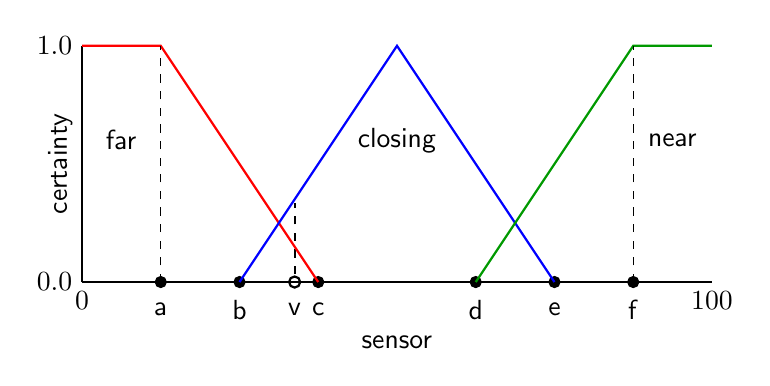
\begin{tikzpicture}
\draw (0,0) node[left] {\p{0.0}} node[below] {\p{0}} -- node[sloped,above] {\textsf{certainty}} (0,3) node[left] {\p{1.0}};
\draw (0,0) -- node[below,yshift=-16pt] {\textsf{sensor}} (8,0) node[below] {\p{100}};
\foreach \n/\x in {a/1,b/2,c/3,d/5,e/6,f/7} {
  \draw[fill] (\x,0) circle [radius=2pt];
  \node at (\x,-10pt) { \textsf{\n} };
}
\draw[thick] (2.7,0) circle [radius=2pt];
\node at (2.7,-10pt) { \textsf{v} };
\draw[dashed,thick] (2.7,.1) -- +(0,.9);
\draw[red,thick] (0,3) -- (1,3) -- (3,0);
\draw[blue,thick] (2,0) -- (4,3) -- (6,0);
\draw[green!60!black,thick] (5,0) -- (7,3) -- (8,3);
\draw[dashed] (1,0) -- (1,3);
\draw[dashed] (7,0) -- (7,3);
\node at (.5,1.8) {\textsf{far}};
\node at (4,1.8) {\textsf{closing}};
\node at (7.5,1.8) {\textsf{near}};
\end{tikzpicture}
\caption{Fuzzify the value of the horizontal proximity sensor}\label{fig.fuzz}
\end{center}
\end{figure}

The labeled points on the $x$-axis refer to thresholds: (a) \p{far\_low}, (b) \p{closing\_low}, (c) \p{far\_high}, (d) \p{near\_low}, (e) \p{closing\_high}, (f) \p{near\_high}. If the value of the sensor is below \p{far\_low}, then we are completely certain that the object is far away and the certainty is $1$. If the value is between \p{closing\_low} and \p{far\_high} then we are somewhat certain that the object is far away, but also somewhat certain that it is closing. The fuzziness results from the overlapping ranges: when the value is between point (b) and point (c), we can't say with complete certainty if the object is far away or closing. For the sensor value \p{v} of about $33$ the certainty of \p{far} is about $.15$ and the certainty of \p{closing} is about $.25$.

\section{Apply rules}

The three premises, the certainties of \p{far}, \p{closing} and \p{near}, are used to compute five consequents\index{fuzzy logic!consequent} using the following rules\index{fuzzy logic!rule}:

\begin{enumerate}
\item If \p{far} then \p{very fast}
\item If \p{far} and \p{closing} then \p{fast}
\item If \p{closing} then \p{cruise}
\item If \p{closing} and \p{near} then \p{slow}
\item If \p{near} then \p{stop}
\end{enumerate}

The certainties of the consequents resulting from rules 1, 3, 5 are the same as the certainties of the corresponding premises. When there are two premises, as in rules 2 and 4, the certainties of the consequents are computed from the minimum of the certainties of the premises. Since \emph{both} of the premises must apply, we can't be \emph{more certain} of the consequent than we are of the smaller of the premises. For the value \p{v} in Fig.~\ref{fig.fuzz}, rule 2 applies and the certainty of the consequent is $\min(.15,.25)=.15$.

Another way of combining premises is to take their joint probability:
\[
p(A \cap B) = P(A)\cdot P(B)\,.
\]
For value \p{v}, the certainty of the consequent is $.15\times .25= .0375$, much less than the certainty obtained from the minimum function.

\section{Defuzzify}

The next step is to combine the consequents, taking into account their certainties. Figure~\ref{fig.defuzz} shows the output motor powers for each of the five consequents. For example, if we are completely certain that the output is \p{cruise}, the center graph in the figure shows that the motor power should be set to $50$, but if we were less certain, the motor power should be less or more.

\begin{figure}
\begin{center}
% Defuzzify to obtain a crisp motor setting
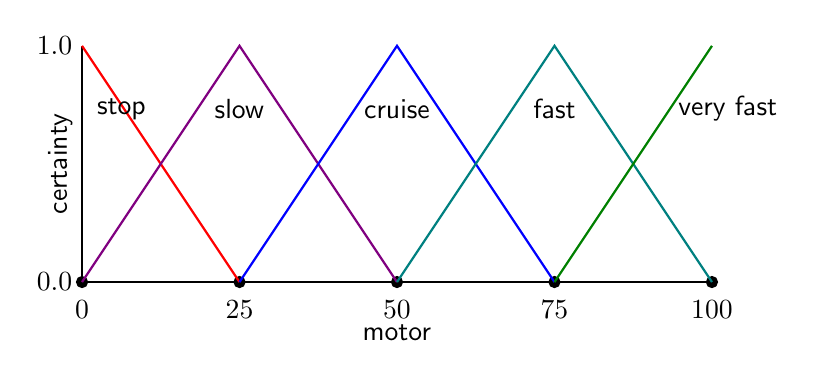
\begin{tikzpicture}
\draw (0,0) node[left] {\p{0.0}} -- node[sloped,above] {\textsf{certainty}} (0,3) node[left] {\p{1.0}};
\draw (0,0) -- node[below,yshift=-12pt] {\textsf{motor}} (8,0);
\foreach \n/\x in {0/0,25/2,50/4,75/6,100/8} {
  \draw[fill] (\x,0) circle [radius=2pt];
  \node at (\x,-10pt) { \p{\n} };
}
\draw[red,thick] (0,3) -- (2,0);
\draw[red!50!blue,thick] (0,0) -- (2,3) -- (4,0);
\draw[blue,thick] (2,0) -- (4,3) -- (6,0);
\draw[blue!50!green,thick] (4,0) -- (6,3) -- (8,0);
\draw[green!50!black,thick] (6,0) -- (8,3);
\node at (.5,2.2) {\textsf{stop}};
\node at (2,2.2) {\textsf{slow}};
\node at (4,2.2) {\textsf{cruise}};
\node at (6,2.2) {\textsf{fast}};
\node at (8.2,2.2) {\textsf{very fast}};
\end{tikzpicture}
\caption{Defuzzify to obtain the crisp motor setting}\label{fig.defuzz}
\end{center}
\end{figure}

Suppose that the certainty of the consequent of \p{cruise} is computed to be $0.4$. Then the center triangle in Fig.~\ref{fig.defuzz} is no longer relevant because the certainty can never be more than $0.4$, which is displayed as a trapezoid in Fig.~\ref{fig.trap}.

\begin{figure}
\begin{center}
% Areas defined by the certainties of the consequents
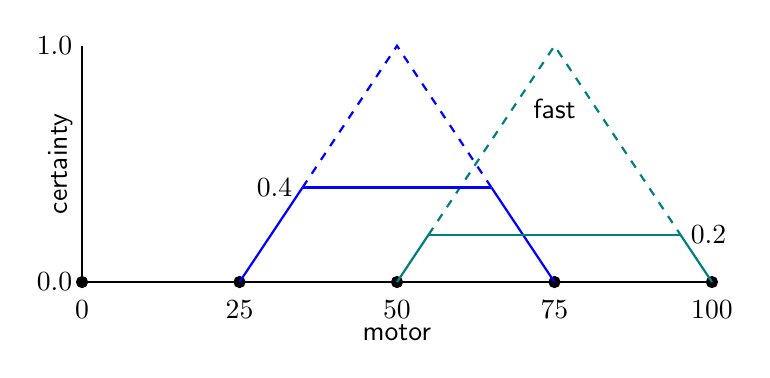
\begin{tikzpicture}
\draw (0,0) node[left] {\p{0.0}} -- node[sloped,above] {\textsf{certainty}} (0,3) node[left] {\p{1.0}};
\draw (0,0) -- node[below,yshift=-12pt] {\textsf{motor}} (8,0);
\foreach \n/\x in {0/0,25/2,50/4,75/6,100/8} {
  \draw[fill] (\x,0) circle [radius=2pt];
  \node at (\x,-10pt) { \p{\n} };
}
\draw[blue,thick] (2,0) -- (2.8,1.2);
\draw[blue,thick] (5.2,1.2) -- (6,0);
\draw[blue,thick,dashed] (2.8,1.2) -- (4,3) -- (5.2,1.2);
\draw[blue!50!green,thick] (4,0) -- (4.4,.6);
\draw[blue!50!green,thick] (7.6,.6) -- (8,0);
\draw[blue!50!green,thick,dashed] (4.4,.6) -- (6,3) -- (7.6,.6);
node at (4,2.2) {\textsf{cruise}};
\node at (6,2.2) {\textsf{fast}};
\draw[blue,thick] (2.8,1.2) node[black,left] {\p{0.4}} -- (5.2,1.2);
\draw[blue!50!green,thick] (4.4,.6) -- (7.6,.6) node[black,right] {\p{0.2}};
\end{tikzpicture}
\caption{Areas defined by the certainties of the consequents}\label{fig.trap}
\end{center}
\end{figure}

Let $w$ and $h$ be the width and height of a triangle. Then the area of a trapezoid bounded by the line at height $h'$ is given by the formula:\footnote{The derivation of the formula is given in Appendix~\ref{a.trap}.}
\begin{displaymath}
wh'\left(1-\frac{h'}{2h}\right)\,.
\end{displaymath}
It is possible that more than one consequent has positive values. Figure~\ref{fig.trap} shows the trapezoids for the consequent \p{cruise} with a certainty of $0.4$ and the consequent \p{fast} with a certainty of $0.2$. For $w=50$, $h=1$, $h_{c}'=0.4$ (\p{cruise}), $h_{f}'=0.2$ (\p{fast}), the areas of the trapezoids $a_c$ (\p{cruise}) and $a_f$ (\p{fast}) are:
\begin{displaymath}
\spacearray
\begin{array}{l}
a_c = 50\times 0.4 \left(1 - \frac{0.4}{2}\right) = 16\\
a_f = 50\times 0.2 \left(1 - \frac{0.2}{2}\right) = 9\,.
\end{array}
\end{displaymath}
To obtain a crisp value\index{fuzzy logic!crisp value}, the \emph{center of gravity} is computed. This is the sum of the areas of the trapezoids weighted by the value at the center of the base of each trapezoid divided by the sum of the areas:
\begin{displaymath}
\frac{16\times 50 + 9\times 75}{16+9}=59\,.
\end{displaymath}
The value is closer to the value associated with \p{cruise} than it is to the value associated with \p{fast}. This is not surprising since the certainty of \p{cruise} is greater than the certainty of \p{fast}.

\begin{framed}
\act{Fuzzy logic}{fuzzy}
\begin{itemize}
\item Implement the fuzzy logic controller for a robot approaching an object.
\item Define appropriate thresholds for the proximity sensor and appropriate values for defuzzifying to obtain a crisp motor speed.
\item Compare the results with the proportional control algorithm you implemented in Activity~\ref{act.proportional}.
\end{itemize}
\end{framed}

\section{Summary}

Fuzzy logic control is an alternative to the classical mathematical control algorithms described in Chap.~\ref{ch.control}. The advantage of fuzzy logic control is that it does not demand precise mathematical specifications of the robot's behavior which may be difficult to define. We gave an example of fuzzy definitions of speed; other examples would be color (when does a shade of red become orange?) and temperature (when does a warm room become hot?). The disadvantage is that the behavior of fuzzy logic control is not as transparent as that of classical control algorithms.

\section{Further reading}

The original work on fuzzy logic was done by Lotfi Zadeh \cite{zadeh}. A textbook on the application of fuzzy logic to control is \cite{passino}.  Fuzzy logic is also used in image processing \cite[Sect.~3.8]{GW}.

\bibliographystyle{spmpsci}
\bibliography{er}
